\section{Experiments}
\label{sec:exp}

\paragraph{Setup.}
FakeAVCeleb~\cite{khalid2021fakeavceleb} is split deterministically into $3850$ training, $825$ validation, and $825$ test clips, each with a $1{:}10$ real/fake ratio (real $=0$, fake $=1$). Cross-dataset transfer uses $500$ LAV-DF~\cite{cai2022lavdf} clips. Models are trained with AdamW (learning rate $5\!\times\!10^{-4}$, weight decay $0.01$), batch size $8$ with gradient accumulation $4$, cosine decay with $3$ warmup epochs, gradient clipping $1.0$, and early stopping. Main results average five seeds ($42,69,420,2026,2804$); Phase-2 studies (anisotropic, conformal) use seed $2026$, justified by the low five-seed variance established below. Certification uses $n_0=100$, $n=1000$, $\alpha=0.001$.

\subsection{Isotropic certification}

\begin{table}[t]
\centering
\caption{Joint feature-space certification on FakeAVCeleb (five seeds, mean$\pm$std). C@$r$ is certified accuracy (\%) at radius $r$.}
\label{tab:main}
\footnotesize
\setlength{\tabcolsep}{3pt}
\begin{tabular}{ccccccc}
\toprule
$\sigma$ & Acc. & Abs. & Mean $R$ & C@0.25 & C@0.50 & C@1.0/1.5 \\
\midrule
0.12 & $91.2{\pm}1.0$ & 0.3 & $0.288{\pm}.003$ & 88.8 & 0.0 & 0.0/0.0 \\
0.25 & $91.2{\pm}1.1$ & 0.4 & $0.588{\pm}.012$ & 89.4 & 86.6 & 0.0/0.0 \\
0.50 & $91.5{\pm}1.1$ & 0.4 & $1.165{\pm}.034$ & 90.5 & 89.2 & 85.4/0.0 \\
1.00 & $92.5{\pm}0.6$ & 0.8 & $2.215{\pm}.032$ & 91.8 & 90.7 & 88.0/84.9 \\
\bottomrule
\end{tabular}
\end{table}

\begin{figure}[t]
\centering
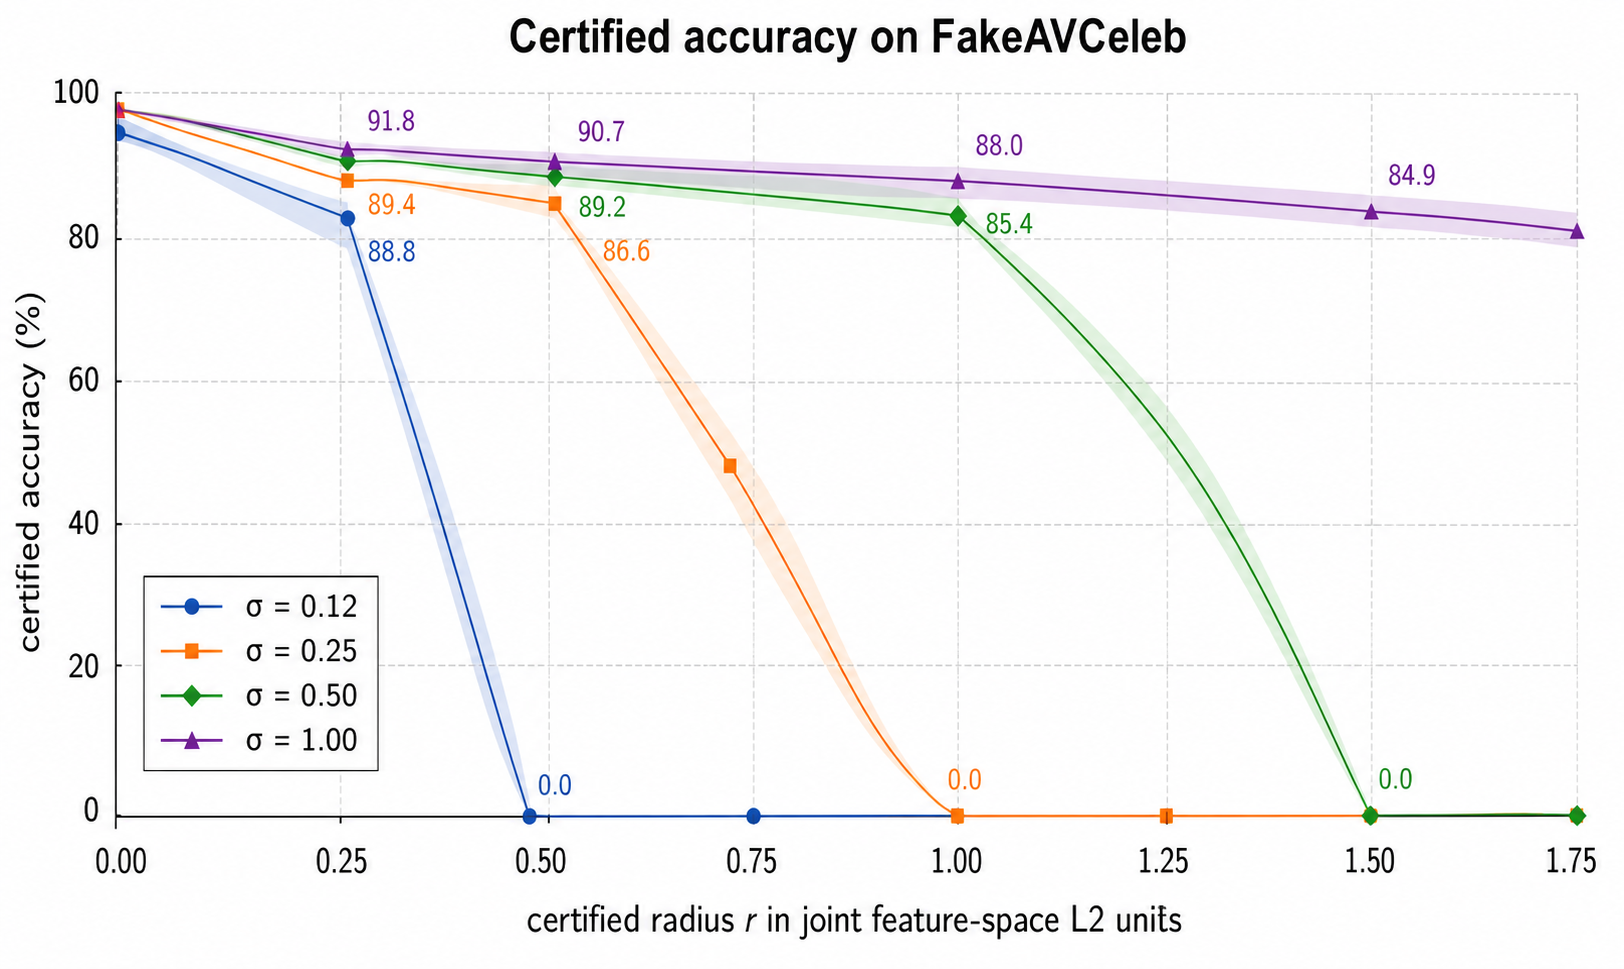
\includegraphics[width=\linewidth]{figures/certified_accuracy_curves.png}
\caption{Certified accuracy vs.\ radius. Larger $\sigma$ shifts the curve right; the $\sigma=1.0$ model retains high certified accuracy through radius $1.5$.}
\label{fig:curves}
\end{figure}

Table~\ref{tab:main} reports the headline isotropic result. Larger smoothing noise increases the certified radius \emph{without} reducing clean accuracy, and abstention never exceeds $1\%$ --- both unusual for randomized smoothing and both explained by Theorem~\ref{thm:scaling}: the classifier sees only the on-manifold noise $\sigma\sqrt{d}$, so the margin is preserved while the radius grows with $\sigma$. The five-seed standard deviations are small ($\pm0.6\%$ accuracy, $\pm0.032$ radius at $\sigma=1.0$), which justifies single-seed Phase-2 studies. Figure~\ref{fig:curves} shows the full certified-accuracy curves.

\subsection{Geometry, not training, drives certifiability}

\begin{table}[t]
\centering
\caption{Baselines at $\sigma=1.0$. The no-noise model certifies within $1.9\%$ of the noise-trained model; feature-space PGD-AT inflates the radius but collapses validation AUC.}
\label{tab:baselines}
\footnotesize
\setlength{\tabcolsep}{3.2pt}
\begin{tabular}{lccccc}
\toprule
Model & Val AUC & EER & Acc. & Mean $R$ & C@1.0/1.5 \\
\midrule
Joint noise & $0.941$ & $0.139$ & 92.5 & 2.215 & 88.0/84.9 \\
No-noise & $0.877$ & $0.194$ & 92.3 & 2.173 & 86.3/82.0 \\
PGD-AT & $0.730$ & $0.335$ & 90.5 & 2.463 & 90.5/90.5 \\
\bottomrule
\end{tabular}
\end{table}

Table~\ref{tab:baselines} isolates the role of training. The no-noise baseline reaches mean radius $2.173$, only $1.9\%$ below the noise-trained $2.215$ --- exactly as Remark~\ref{rem:effnoise} predicts, since the frozen geometry fixes $d/D$ and only the margin can be tuned. Feature-space PGD adversarial training (PGD-AT) attains a larger radius ($2.463$) but its validation AUC collapses from $0.941$ to $0.730$ (EER $0.139\!\to\!0.335$): it trivially stabilizes predictions by flattening the decision boundary, certifying everything at the cost of discrimination. CertAV should thus not be read as an adversarial-training recipe; its value is to expose and certify a favorable geometry already present in frozen representations.

\subsection{Encoder-scaling study}

\begin{table}[t]
\centering
\caption{Five encoder families (no-noise baseline, $\sigma=1.0$). $d$ is the $90\%$-variance PCA dimension; $\mathcal{A}=\sqrt{D/d}$. Lower $d/D$ tracks larger $\bar R$.}
\label{tab:encoder}
\footnotesize
\setlength{\tabcolsep}{3.5pt}
\begin{tabular}{lcccccc}
\toprule
Encoder pair & $D$ & $d$ & $d/D$ & $\mathcal{A}$ & $\bar R$ & Acc. \\
\midrule
DINOv2-S + WavLM        & 1152 & 80  & 0.069 & 3.79 & 2.207 & 90.8 \\
DINOv2-S + HuBERT       & 1152 & 79  & 0.069 & 3.82 & 2.173 & 90.2 \\
DINOv2-B + Whisper-base & 1280 & 119 & 0.093 & 3.28 & 2.132 & 92.2 \\
DINOv2-S + Whisper-tiny &  768 & 80  & 0.104 & 3.10 & 2.190 & 91.4 \\
CLIP-B + Whisper-tiny   & 1152 & 126 & 0.109 & 3.02 & 1.948 & 94.3 \\
\bottomrule
\end{tabular}
\end{table}

\begin{figure}[t]
\centering
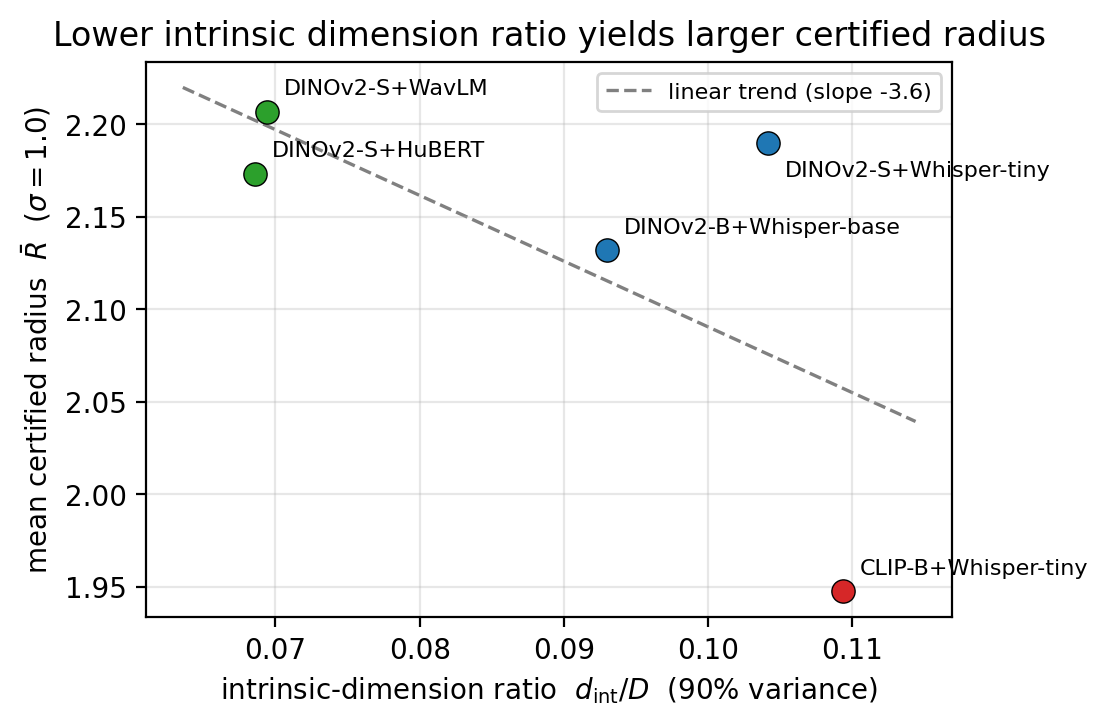
\includegraphics[width=\linewidth]{figures/encoder_scaling_scatter.png}
\caption{Encoder scaling. Self-supervised audio encoders (WavLM, HuBERT) give the lowest $d/D$ and largest radii; the contrastive CLIP visual encoder gives the highest $d/D$ and the smallest radius despite the best clean accuracy.}
\label{fig:scatter}
\end{figure}

Table~\ref{tab:encoder} and Figure~\ref{fig:scatter} test Corollary~\ref{cor:amp} across five pairs combining DINOv2~\cite{oquab2024dinov2}, CLIP~\cite{radford2021clip}, Whisper~\cite{radford2023whisper}, HuBERT~\cite{hsu2021hubert}, and WavLM~\cite{chen2022wavlm}. The trend predicted by the theory holds at the extremes: the lowest-$d/D$ pairs (DINOv2-S\,+\,WavLM/HuBERT, $d/D\!\approx\!0.069$) achieve the largest radii ($\bar R\!\approx\!2.2$), while CLIP-B\,+\,Whisper-tiny ($d/D\!=\!0.109$) achieves the smallest ($1.948$) \emph{despite} the highest clean accuracy ($94.3\%$). The ordering is not strictly monotone in the mid-range, so $d/D$ is the dominant but not the sole predictor --- spectral decay rate and feature non-Gaussianity likely also contribute, and we therefore claim a dominant trend rather than an exact functional law. The accuracy/certifiability trade-off is itself useful guidance: contrastive encoders favor clean accuracy, self-supervised encoders favor certifiability.

\subsection{Manifold-aware anisotropic smoothing}

\begin{table}[t]
\centering
\caption{Anisotropic smoothing at equalized budget $\mathrm{trace}(\Sigma)=D\sigma^2$ ($\sigma=1.0$, seed $2026$). $R_{\Smanifold}$ is the on-manifold radius; $R_{\ell_2}$ the worst-case radius. For anisotropic rows, $\mathrm{C}_{\Smanifold}$@1.0 is certified accuracy w.r.t.\ the on-manifold radius $R_{\Smanifold}$, \emph{not} the worst-case $R_{\ell_2}$ (the two coincide for the isotropic row); it is therefore not a like-for-like comparison with the isotropic $88.0$, but the appropriate metric under a manifold-aware threat model. Strategy~2 gives the largest $R_{\Smanifold}$ and zero abstention.}
\label{tab:aniso}
\footnotesize
\setlength{\tabcolsep}{3pt}
\begin{tabular}{lccccc}
\toprule
Strategy & Acc. & Abs. & $R_{\ell_2}$ & $R_{\Smanifold}$ & $\mathrm{C}_{\Smanifold}$@1.0 \\
\midrule
Isotropic & 90.9 & 0.8 & 2.215 & 2.215 & 88.0 \\
S1: eigenvalue-prop. & 90.9 & 0.7 & 0.0002 & 6.272 & 89.5 \\
\textbf{S2: subspace proj.} & \textbf{90.9} & \textbf{0.0} & 0.0025 & \textbf{7.632} & \textbf{90.9} \\
S3: inverse-eigenvalue & 90.9 & 0.7 & 0.0139 & 6.586 & 89.0 \\
\bottomrule
\end{tabular}
\end{table}

\begin{figure}[t]
\centering
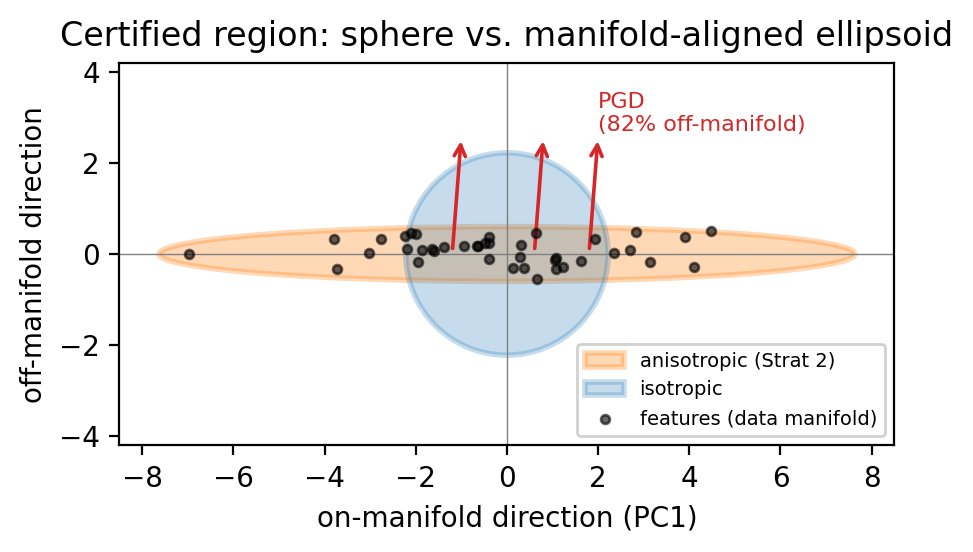
\includegraphics[width=0.92\linewidth]{figures/sphere_vs_ellipsoid.png}
\caption{Isotropic smoothing certifies a sphere (radius $2.22$, equal in all directions); manifold-aware smoothing (S2) certifies an ellipsoid with on-manifold axis $7.63$ and near-zero off-manifold axes. PGD attacks point $82\%$ off-manifold ($\cos^2\theta\!\approx\!0.18$), where the classifier is provably invariant.}
\label{fig:ellipse}
\end{figure}

Table~\ref{tab:aniso} reports the three strategies of Sec.~\ref{ssec:aniso} at \emph{equalized} budget; the improvement is purely from redistribution. Strategy~2 (subspace projection) achieves an on-manifold radius of $7.63$, a $3.4\times$ lift over isotropic ($2.22$), and attains $0\%$ abstention --- every correctly classified clip is certified, because concentrating noise inside $\Smanifold$ minimizes what the classifier head sees and maximizes $p_A$. The near-zero $R_{\ell_2}$ is \emph{by design} (Fig.~\ref{fig:ellipse}): the certificate is an ellipsoid with long axes in the $80$ on-manifold directions and tiny axes in the $688$ off-manifold directions where the classifier is invariant. Under a manifold-aware threat model --- the relevant one, given $\cos^2\theta\!\approx\!0.18$ --- the on-manifold radius is the correct adversarial metric, and an attacker spreading budget uniformly faces an even larger effective barrier since most energy lands off-manifold. This is the paper's headline result.

\subsection{Robust conformal prediction}

\begin{table}[t]
\centering
\caption{Split conformal prediction on the $\sigma=1.0$ model ($\alpha=0.10$, seed $2026$). Marginal coverage and singleton rate are stable under PGD; class-conditional coverage exposes the $1{:}10$ imbalance.}
\label{tab:conformal}
\footnotesize
\setlength{\tabcolsep}{4pt}
\begin{tabular}{lcccc}
\toprule
Setting & Cover. & Single. & Cov(real) & Cov(fake) \\
\midrule
Clean & 96.8 & 92.4 & 72.0 & 99.3 \\
PGD $\varepsilon{=}0.25$ & 96.2 & 91.3 & 66.7 & 99.2 \\
PGD $\varepsilon{=}0.50$ & 95.3 & 91.2 & 58.7 & 98.9 \\
PGD $\varepsilon{=}1.00$ & 94.7 & 88.2 & 54.7 & 98.7 \\
\bottomrule
\end{tabular}
\end{table}

Table~\ref{tab:conformal} reports conformal prediction at the primary operating point $\alpha=0.10$. Standard split conformal achieves target marginal coverage ($>90\%$) on clean data and degrades gracefully under PGD (to $94.7\%$ at $\varepsilon=1.0$). The robust variant of Gendler et al.~\cite{gendler2022adversarially} restores guaranteed coverage by enlarging sets: at $r\ge 0.25$ the calibrated threshold reaches $0.5$, so every set becomes $\{\text{real},\text{fake}\}$ --- $100\%$ coverage at $0\%$ efficiency. This is the fundamental coverage-efficiency trade-off, and we therefore report $\alpha=0.10$ as the operating point rather than the conservative $\alpha=0.05$. Marginal coverage meets the $1-\alpha$ target throughout, but conditional coverage varies sharply by class: fake clips (majority) are covered near-perfectly ($>98\%$) while real clips (minority) are covered far less ($54.7$--$72.0\%$). This deserves emphasis rather than a footnote, because the ``real'' class is the safety-critical one --- under-covering it corresponds to false deepfake accusations of genuine media. The gap is a known property of \emph{marginal} split conformal under class imbalance~\cite{romano2020classification} and is intrinsic to the dataset's $1{:}10$ ratio, not to our use of it; the standard remedy is \emph{class-conditional} (Mondrian) calibration, which enforces the coverage target within each class at the cost of wider ``real'' sets, and which we leave as the natural next step. We report marginal coverage here for comparability with prior work and flag the conditional gap explicitly. Crucially, even with this caveat, conformal prediction returns a covered set for the samples on which CertAV abstains, which is the practical complement to the per-sample certificate.

\subsection{Modality, transfer, and degradation}

\begin{table}[t]
\centering
\caption{Modality ablation (five seeds). Unimodal certificates can match or exceed joint radii but protect a strictly smaller threat set.}
\label{tab:modality}
\footnotesize
\setlength{\tabcolsep}{4pt}
\begin{tabular}{lccccc}
\toprule
Mode & $\sigma$ & Acc. & Mean $R$ & C@0.25 & C@0.50 \\
\midrule
Joint       & 0.25 & 91.2 & 0.588 & 89.4 & 86.6 \\
Visual-only & 0.25 & 91.0 & 0.589 & 89.3 & 86.5 \\
Audio-only  & 0.25 & 90.9 & 0.607 & 90.3 & 89.5 \\
\midrule
Joint       & 1.00 & 92.5 & 2.215 & 91.8 & 90.7 \\
Visual-only & 1.00 & 92.3 & 2.273 & 91.6 & 90.7 \\
Audio-only  & 1.00 & 91.9 & 2.404 & 91.7 & 91.5 \\
\bottomrule
\end{tabular}
\end{table}

\begin{table}[t]
\centering
\caption{Transfer and degradation at $\sigma=1.0$. LAV-DF is cross-dataset; degradations are on FakeAVCeleb.}
\label{tab:transfer}
\footnotesize
\setlength{\tabcolsep}{4pt}
\begin{tabular}{lcccc}
\toprule
Setting & Acc. & Mean $R$ & C@0.50 & C@1.0 \\
\midrule
LAV-DF transfer    & 74.6 & 1.626 & 69.2 & 61.4 \\
Social degradation & 91.3 & --    & 90.5 & -- \\
H.264 CRF 28       & 90.7 & --    & 89.9 & -- \\
JPEG quality 75    & 91.6 & --    & 90.5 & -- \\
\bottomrule
\end{tabular}
\end{table}

Table~\ref{tab:modality} shows that audio-only smoothing at $\sigma=1.0$ has the largest mean radius ($2.404$), but it leaves the visual stream outside the certified set; the joint certificate is the more conservative statement when either modality may be manipulated. Table~\ref{tab:transfer} reports cross-dataset and degradation robustness: on LAV-DF the certificate transfers at $74.6\%$ accuracy and $61.4\%$ certified accuracy at radius $1.0$ --- useful but imperfect, confirming dataset shift as a real limitation --- while common media degradations (social re-encoding, H.264, JPEG) preserve $\ge 90\%$ certified accuracy at radius $0.5$.

\paragraph{Composed input-space certificate.}
To address the feature-space scope head-on, we estimate the empirical feature-to-input Lipschitz constant from input-space attacks: the measured displacement-to-perturbation ratio is tightly concentrated at $L\!\approx\!50$ across attack magnitudes. Composing $R_{\mathrm{cert}}/L$ maps the feature certificate to an \emph{approximate} input-space radius of $\approx\!0.12$, at which $\approx\!90.7\%$ of clips remain correct and certified. This is an empirical, probabilistic bridge --- not a worst-case formal Lipschitz proof --- but it gives a concrete sense of the input-space protection the certificate implies, and the methodology composes directly with any future formal encoder bound.
